We've observed above that the sum of cosines is preserved for the family of orbits as well as the product of cosines for the family of tangential orbits.

Consider more generally, two calculations applicable to all trajectories, closed or not:

\begin{itemize}
    \item $K$ the arithmetic mean of cosines
    \item $K'$ the geometric mean of tangential cosines
\end{itemize}

Parametrize a trajectory family by the minor semiaxis $\beta$ of their confocal caustic, Figure~\ref{fig:gen-caustic-pencil}. Asymptotically:

\begin{eqnarray}
K(\beta)&=&\lim_{M\to\infty}\,\,\frac{1}{M}\,  \sum_{i=1}^{M}{\cos\theta_i}\\
K'(\beta)&=&\lim_{M\to\infty}|\prod_{i=1}^{M}{\cos\theta_i'}|^{1/M}
\end{eqnarray}

Where $\theta_i$ (resp. $\theta_i'$) are the angles between consecutive segments of the trajectory (resp. tangential polygon). For trajectories which do not close, the above will not depend on the starting point on the ellipse (trajectories are space-filling, Figure~\ref{fig:space-filling}). The above expressions become equivalent to the following spatial integrals, whose density depends on $\kappa(s)$, the curvature of the caustic parametrized by arc length \cite{sergei17_curvature}:

\begin{figure}
    \centering
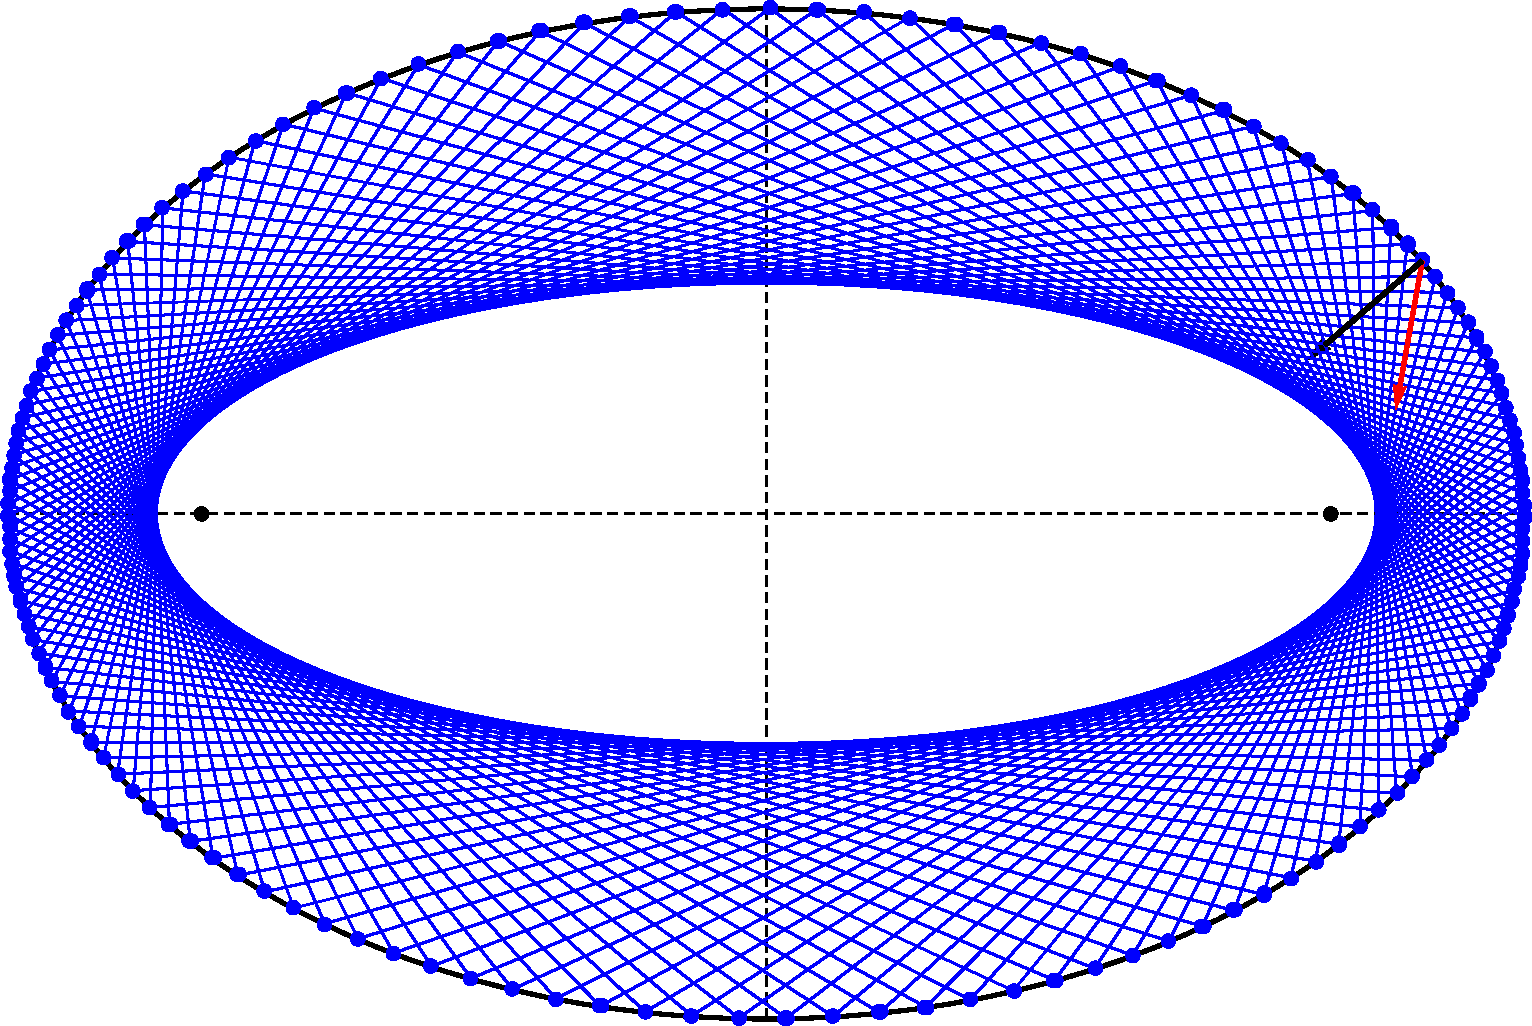
\includegraphics[width=.5\textwidth]{pics/0210_space_filling.pdf}
    \caption{300 edges of a  space-filling trajectory (the starting location and direction is shown by a red arrow on the Billiard's first quadrant.}
    \label{fig:space-filling}
\end{figure}

\begin{eqnarray}
K(\beta)&=&\frac{1}{\Delta}\,\,\oint\,\cos\theta\,\kappa(s)^{2/3}ds\\
\log K'(\beta)&=&\frac{ 1}{\Delta}\,\,\oint \,\log|\cos\theta'|\,\kappa(s)^{2/3}ds\\
\mbox{with}\,\Delta&=&\oint\,\kappa(s)^{2/3}ds
\end{eqnarray}

\begin{figure}
    \centering
    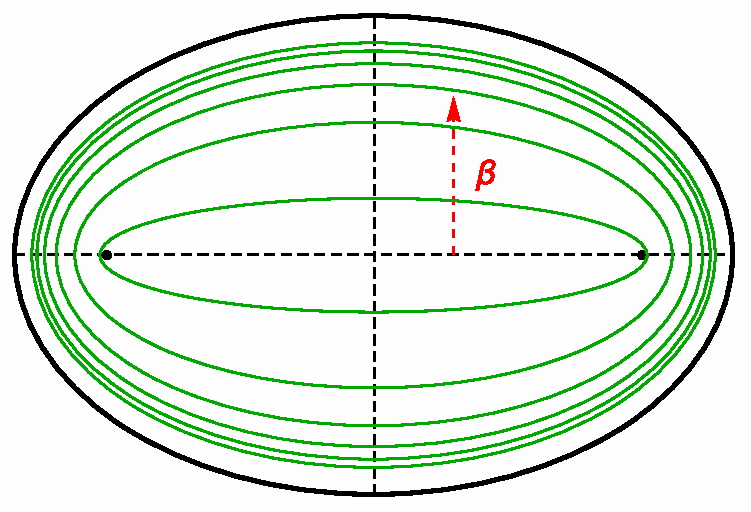
\includegraphics[width=.5\textwidth]{pics/0175_caustic_pencil.pdf}
    \caption{An $a=1.5$ billiard is shown as well as a few members (green) of a continuous pencil of confocal caustics, parametrized by $\beta\in(0,1)$, their minor semiaxis.}
    \label{fig:gen-caustic-pencil}
\end{figure}

These spatial averages  are shown in Figure~\ref{fig:koiller-sum-prod} for $a=5$ (smaller $a$ make the two spatial averages become to close to each other). For values of $\beta$ where the trajectory becomes close, the spatial averages yield numbers which perfectly match mean cosines and geometric mean excentral cosines when these are estimated numerically over an orbit family (not via the integral). It appears that for any $a$, $|K|>K'$.

\begin{figure}
    \centering
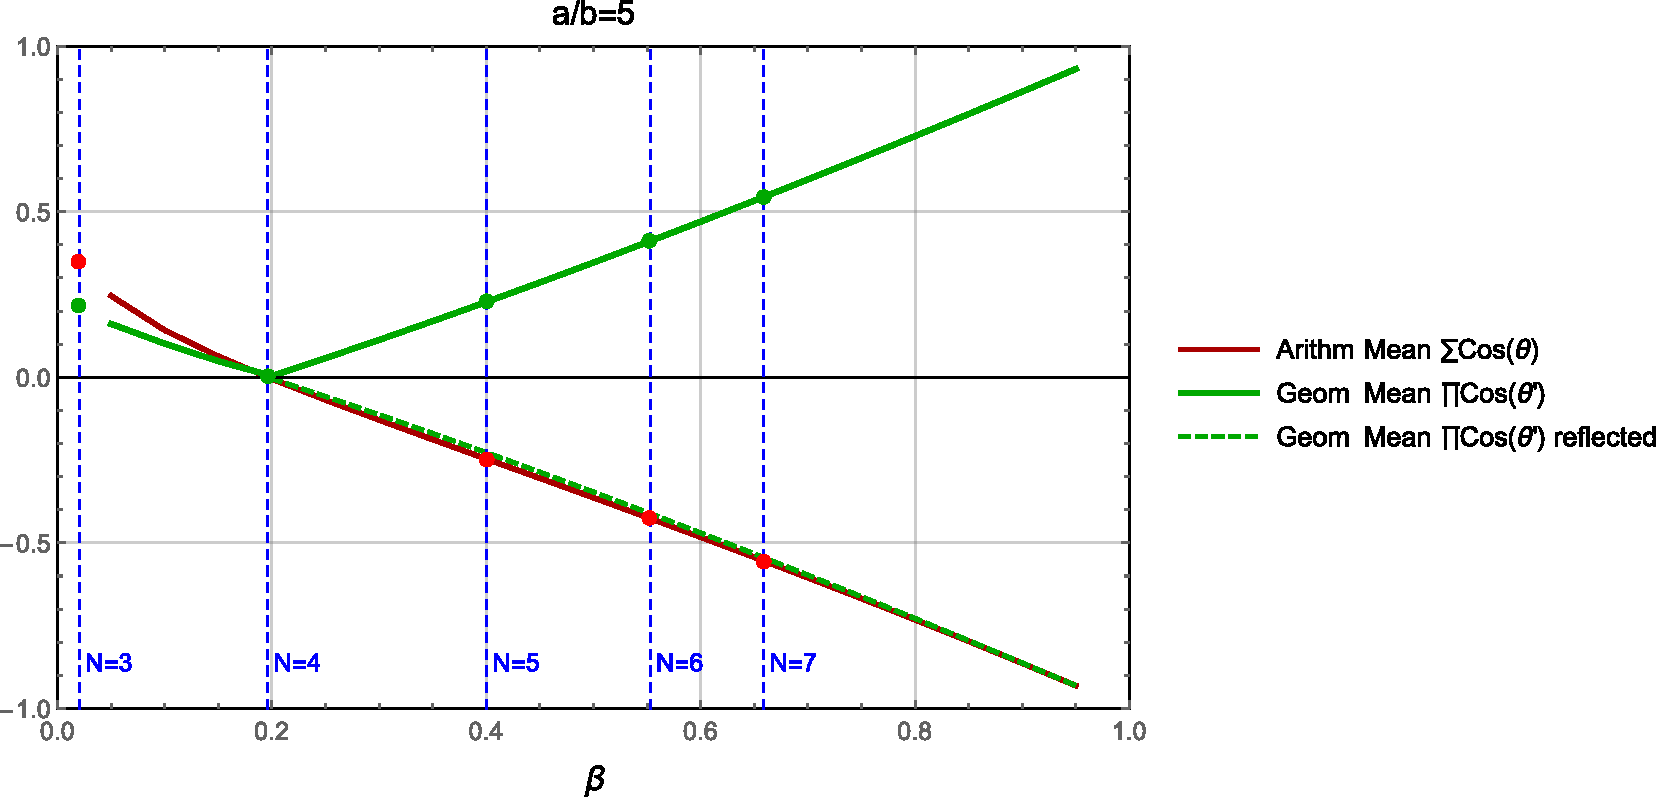
\includegraphics[width=\textwidth]{pics/0172_koiller_sum_prod_a5.pdf}
    \caption{Spatial Averages vs. $\beta$, the caustic minor semiaxis, for $a=5$. Blue dashed vertical lines mark the $\beta$ for non-intersecting orbits. Red: $K$, the arithmetic mean of trajectory cosines. Green: $K'$, the geometric mean of tangential cosines. Dashed green: past the $N=4$ caustic, the $K'$ curve is reflected about the $x$ axis to show it closely tracks $K$ (though they are never the same). Blue and red dots are the same averages obtained via closed-form expressions, perfectly matching the spatial average curves.}
    \label{fig:koiller-sum-prod}
\end{figure}
